\documentclass[9pt]{exam} 
\addpoints
\pointsinmargin

\usepackage[fleqn]{amsmath}
\usepackage{amssymb} %standard classy maths symbols
\usepackage[a4paper, margin=2cm]{geometry} %makes it easy to specify where to put stuff on the page

\usepackage{tcolorbox} % basic but good package for boxes around text
\tcbset{colback=black!5!white}

\usepackage{tikz} % interval diagrams, sets, etc.

\begin{document}


\vspace{-5mm}

\begin{center}
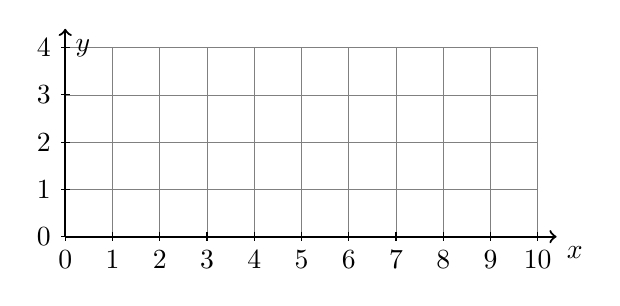
\begin{tikzpicture}[scale=0.6]

% Draw the grid
\draw[step=1cm,gray,very thin] (0,0) grid (10,4);

% Draw the x-axis
\draw[thick,->] (0,0) -- (10.4,0) node[anchor=north west] {$x$};

% Draw the y-axis
\draw[thick,->] (0,0) -- (0,4.4) node[anchor=north west] {$y$};

% Labels for the axes
\foreach \x in {0,1,...,10} \draw (\x,0.1) -- (\x,-0.1) node[anchor=north] {\x};
\foreach \y in {0,1,...,4} \draw (0.1,\y) -- (-0.1,\y) node[anchor=east] {\y};

\end{tikzpicture}
\end{center}



\begin{questions} 
\question[4] Let $\{\overrightarrow{e_1}$, $\overrightarrow{e_2}\}$ be the standard basis. Represent $\overrightarrow{e_1}$, $\overrightarrow{e_2}$, $\overrightarrow{OX}$, and $\overrightarrow{OY}$ above, for $X(7, 1)$ and $Y(2, 3)$.

\question[4] Rewrite and simplify the following vectors using column notation :

\

\begin{parts}
\part $\overrightarrow{OX}$ = \dotfill

\

\part $\overrightarrow{XY}$ = \dotfill

\

\part $\overrightarrow{YX} + 2 \overrightarrow{YO}$ = \dotfill
\fillwithdottedlines{10mm}
\end{parts}

\question[3] Compute the angle $\widehat{XOY}$.
\fillwithdottedlines{\stretch{1}}

\question[3] Compute the coordinates of $Z$ so $OXZY$ is a parallelogram.
\fillwithdottedlines{\stretch{1}}

\question[3] Establish $S_{45^\circ}$ the matrix of a reflection of $45^\circ$, then use matrix multiplication to calculate $\overrightarrow{OR} = S_{45^\circ} (\overrightarrow{OY})$.
\fillwithdottedlines{\stretch{1}}

\question[0] \textbf{Bonus.} 
What is the height of $\triangle OXY$ if $[OX]$ is the base?
\hfill \emph{Work on the back.}

\end{questions}


\begin{tcolorbox}

\textbf{Name of marker:}

\begin{center}
\gradetable[h][questions]
\end{center}

\end{tcolorbox}


\end{document}